Design and Methods

% Weak Scalability Design : Keep Pipeline of Ensembles to show barrier needed in S5 and S6
% Performance, generality with weak scaling (agnostic to kernel)
% Added functionality (do not speak about binding adaptivity to performance or generality)
% In use case: add in why TIES is challenging, and why adaptivity is challenging

% add in pseudo plots for weak, strong, 

For both free energy protocols ESMACS and TIES, each protocol instance
represents a single EnTK pipeline. Both protocols requires a new pipeline to
study each physical system. \jhanote{the above two sentences need to be
clarified. not sure why they are in the experiments section.} Pipelines are
executed concurrently. For the TIES protocol, each pipeline consists of six
stages. EnTK manages the queueing of the tasks in accordance with the order
and concurrency mandated by stages and pipelines. \jhanote{.. need clean
separation of implementation details from design of experiments} Each of the simulation
stages contains a task for every unique $\lambda$-replica combination. 

In the non-adaptive workflow scenario, the first 11 $\lambda$ windows consist
of the following values: $L$ is a vector with
\begin{flalign}
L &= \{ x_i: x_i\in[0,1]\; and\; x_{i+1} = x_i + \delta \}, where\ \delta\ is\ 0.1.
%&$$L=\{ x_i: x_i\in[0,1]\; and\; x_{i+1} = x_i + \delta \}$$%, where $\delta$ is $0.1$.
\end{flalign}

	We append two additional values on both ends of $L$, completing 13 $\lambda$ 
windows. Each $\lambda$ window consists of five replicas. Therefore there are 
a total of 65 tasks for every simulation stage. The production simulations stage,
$s4$ executes a four ns simulation duration.  
The analysis stages of the protocol reduce the number of tasks. The 
first analysis task consists of five tasks where each task performs 
an aggregate analysis over all $\lambda$ windows for each replica. The second 
analysis stage consists of one task that aggregates the previous results and 
computes a single average across all replicas.

In the adaptive workflow, over the course of a run we alter the number of $\lambda$ windows being simulated depending on the difference between the $dU/d\lambda$ measured between adjacent windows.
Increasing the number of $\lambda$ windows in regions of rapid change will 
increase the accuracy of the overall integral to a greater to degree than an
arbitrarily placed window.
In order to access the $dU/d\lambda$ values during runtime, we break down
the single production simulation stage from the nonadaptive workflow into
multiple stages for the adaptive workflow.
Each stage in the adaptive workflow produces only 1 ns of simulation.
Once each stage is complete a decision is made as to whether more $\lambda$ windows are required, and if so where they should be placed. 
We start the workflow with only five $\lambda$ parameters that consist of 
the following values:

\begin{flalign}
L &= \{ x_i: x_i\in[0,1]\; and\; x_{i+1} = x_i + \delta \}, where\ \delta\ is\ 0.25.
%&$$L=\{ x_i: x_i\in[0,1]\; and\; x_{i+1} = x_i + \delta \}$$%, where $\delta$ is $0.1$.
\end{flalign}

For every $\lambda$ window we allocate five replicas therefore yielding a 
total of 25 tasks. We run 25 tasks for stages $s1$ through $s4.1$. Between 
stages \texttt{s4.1} and \texttt{s4.3} the number of $\lambda$ windows doubles for 
every stage, which doubles the total number of tasks. The last production simulation 
stage, \texttt{s4.4}, runs for the remaining 2 ns durations. 

\subsubsection{Weak Scaling Experiments}

We previously demonstrated weak scaling of the ESMACS protocol in [ref SC] where 
we showed that a single ESMACS instance could run up to 128 concurrent pipelines. 
In here we expand upon this work to show weak scalability for the TIES protocol 
by growing the number of protocol instances while adhering to the required number of 
pipelines. By design of each protocol, an increase in the number of instances simply 
means an increase in the number of pipelines. Therefore our previous ESMACS experiment 
referenced in [ref SC] already demonstrates the scalability of ESMACS as a growth in 
the number of pipelines.

The first weak scalability experiment demonstrates the behavior of HTBAC, EnTK and 
RP using the multiple instances of the TIES protocol. By design of weak scaling, 
the ratio between the number of pipelines and cores are kept constant. At every scale 
we introduce twice as many protocol instances. The goal is to isolate and understand
the impact of increasing the number of instances, thereby the execution workload.


\begin{figure}
  \centering
   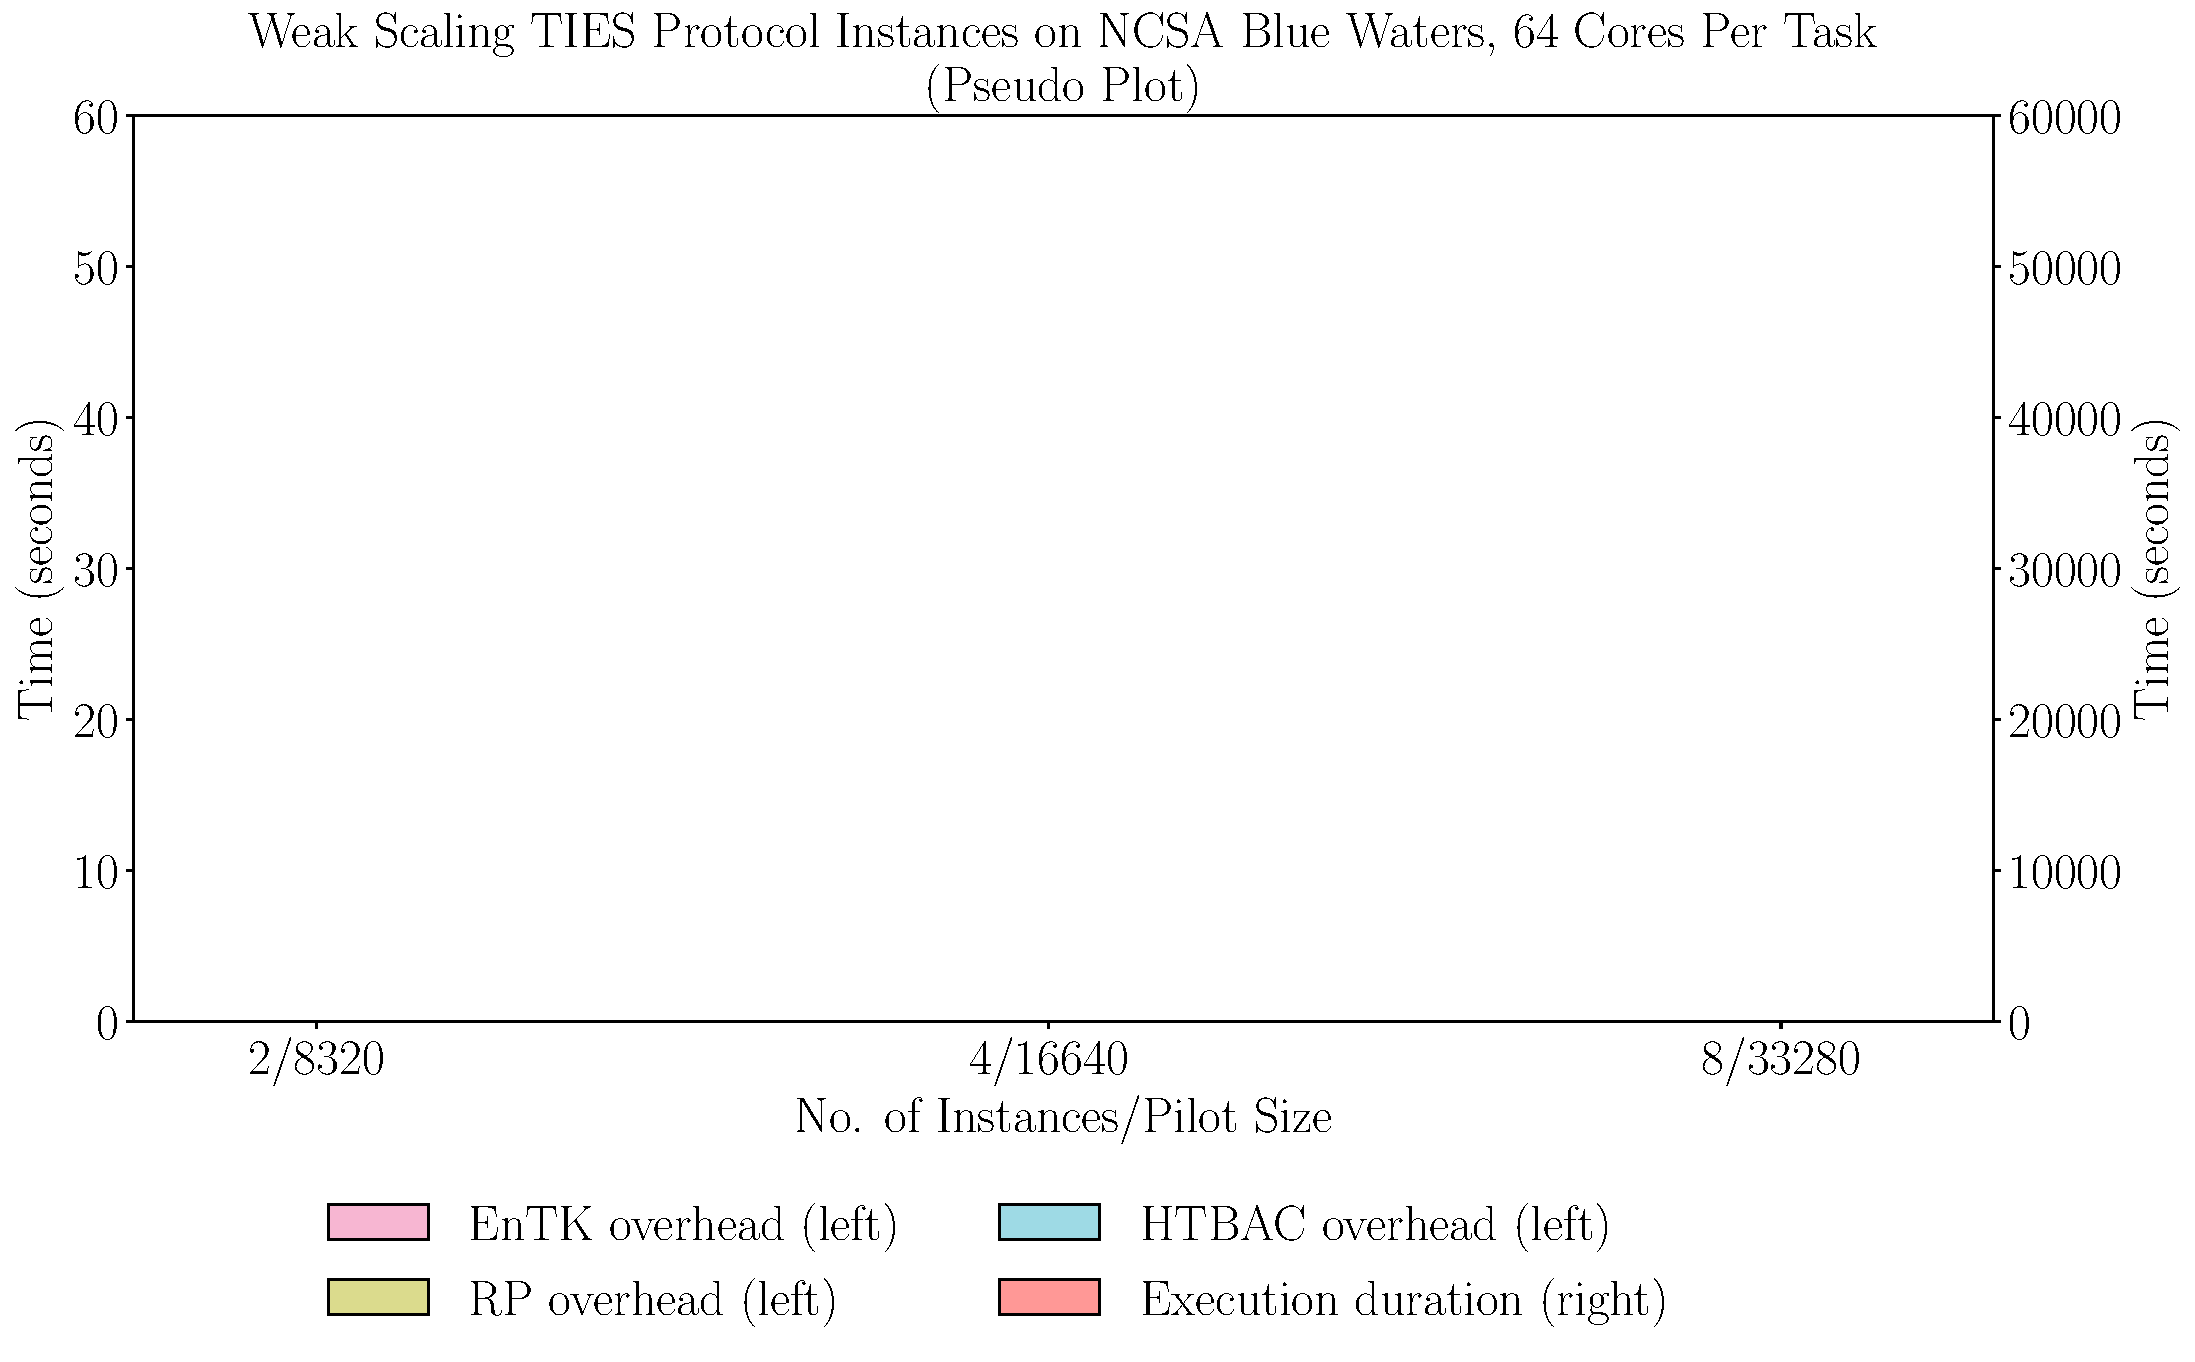
\includegraphics[width=\columnwidth]{figures/weak_scaling_TIES_instances.pdf}
  \caption{Overheads of HTBAC, EnTK, RP when executing weak scaling of TIES. 
  We keep the number of instances and the total number of cores fixed. }
\label{fig:weak_scaling}
\end{figure}


%The next weak scalability experiment replicates the design of the first experiment using a combination of TIES and ESMACS instances. The comparison of experiment 1 and 2 shows the ability to execute procotols with different resource requirements using one pilot.

Strong scalability design: Next we repeat the same design of the weak scalability experiments but examine performance of strong scaling when fixing the number of pipelines and varying the resources. The comparison between weak and strong scalability demonstrates the overhead introduced by load balancing and scheduling tasks in multiple generations.

%Strong scaling argument: If you go big enough you start to encounter high rates of failures on the machines. Part of the reason to do both is to find the sweet spot between weak/strong scaling.

Experimental Setup

We perform weak (and strong) scalability experiments on NCSA Blue Waters--a 13.3. petaFLOPS Cray, with 32 Interlago cores/50 GB RAM per node, Cray Gemini, Lustre shared file system.

Overhead of HTBAC, EnTK and RP

EnTK consists of multiple active components interacting with each other in order to support the execution of ensemble based applications. This process includes various events such as validation of the workflow, validation of the resource description, submission of resource request, creation of tasks, translation of tasks to and from the runtime system amongst several others. In order to understand the contribution of the various events in Ensemble Toolkit, termed as EnTK overhead, to the total time to run, we construct the following experiments.

Time to run = T(overhead\textsubscript{entk}) + T(overhead\textsubscript{rp}) + T(execution)
